% !Mode:: "TeX:UTF-8"

\chapter{构建广义同步数据流图}
\label{chapter-SDF}

\section{COSS 算法简介}
% COSS 流程 及 优劣比较

\subsection{问题模型}

% 首先定义有效调度:
% 包括 任务调度表、消息调度表

首先对目标问题给出一个精确的描述。

(1)	给定一个任务集 $T=\{t_1, t_2, ..., t_n\}$。

(2)	对每个任务 $t_i$,存在两种可能的约束类型:时间约束或数据依赖约束,也可能两种约束都有。

(3)	任务 $t_i$的时间约束是指:任务的释放周期$T_i$、执行的相对时限$D_i$以及首次任务释放时间$O_i$。

(4)	任务的数据依赖约束是指:任务$t_i$与$t_j$之间存在数据依赖关系,每次$t_i$ 执行产生 $p_{ij}$ 个数据发送给 $t_j$ ,而每次 $t_j$ 执行消耗 $c_{ij}$ 个数据。初始时 $t_i$ 到$t_j$的 Delay 为 $D_{ij}$,表示系统启动时在 $t_j$ 第一次运行之前 $t_j$ 在这条依赖关系上有多少数据可用。

(5)	目标平台中处理器数目m(或核数),以及每两个核之间通信时单位时间传输的数据量 s。关于目标平台的抽象模型,在第 \ref{DLS-chapter-SSL} 章有更详细的描述。

针对以上问题,给出一个调度算法,此算法根据以上约束,生成任务集 T 在给定多核架构上的静态周期性调度表以及任务间通信在处理器之间链路上的调度表,使所有任务满足约束条件,或者在调度失败时给出无法调度的结果。



\subsection{算法流程}

% 来自 abstract
COSS 算法主要由三步构成:
\begin{enumerate}
   \item 从表示任务间数据流的 SDF 图构建含有虚拟数据和虚拟结点的广义同步数据流 (General Synchronous Dataflow, GSDF) 图,其同时反映了任务间的数据通信关系和时间约束。
   \item 提出 Improved Class S (ICS) 算法,将上一步中得到的 GSDF 转化为一个调度周期的有向无环图 (Directed Acyclic Graph, DAG),将每个任务的多次执行用不同结点表示,并去除任务间的循环依赖关系。
   \item 提出修改的动态层级调度 (Modified Dynamic Level Scheduling, MDLS) 算法将 DAG 中的任务结点分配至目标多核/处理器平台,得到每个核/处理器的任务调度表,并给出核/处理器之间链路上的通信调度。
 \end{enumerate}

COSS 算法的流程图如图\ref{SDF-fig-COSS-steps}所示。
\begin{figure}[!hbt]
  \centering
  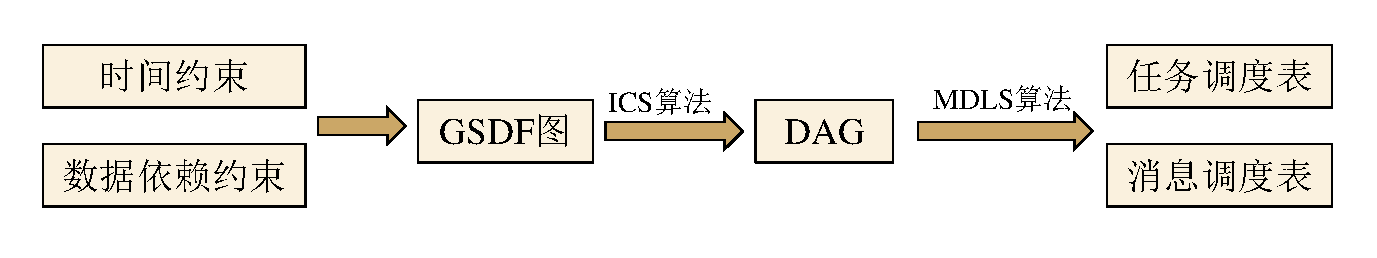
\includegraphics[height=14ex]{figure/SDF-COSS-steps.pdf}
  \caption{COSS 算法流程图}
  \label{SDF-fig-COSS-steps}
\end{figure}



% 来自 SDF改的特点、优势劣势.docx 总结

\subsection{算法特性}

\subsubsection{静态调度}

由离线调度的特征可知,对于实时任务,只能处理周期性任务,而对偶发性任务和非周期任务由于无法预知具体任务的释放时间,无法处理。

离线调度的优势在于,系统开始执行前就排出各个任务的具体调度表,并分配给每个处理器。处理器在具体调度时只需按照分配给自己的调度表执行即可,而不用在运行时占用较大的开销来动态计算调度。每个处理器只用处理自己核上的调度表这一特点和分区调度有些相似,但在允许任务 job-level 迁移的情况时(全局调度)需要处理不同处理器之间任务转移、上下文切换的问题。

离线调度的另一个优势是,调度结果对时间限的保证是容易验证的。尤其对于多处理器的系统,如果将任务间的优先关系放入 WCET 分析中来考虑将带来较大挑战。例如在最简单的分区调度系统上,一个处理器中任务的执行可能间接影响到另外一个处理器上对系统共享资源有竞争关系的另一个任务的执行。有文章指出,目前对这样复杂的硬件相互影响的关系还不存在静态分析方法\upcite{WCET}。


\subsubsection{灵活性}

COSS 算法的本质是将一种周期性和任务间(循环)依赖关系共存的约束转化为一个周期内任务多次执行之间的 DAG 关系,而并没有严格限制只能是分区调度或全局调度。属于分区调度还是全局调度取决于从DAG 到m 个同构多处理器平台的具体映射算法。
如果在映射中限制条件只能将相同任务执行在同一个处理器上,那么将产生分区调度的调度表。如果允许相同任务在不同处理器运行,但每次执行只能在一个处理器上,那么将产生允许 task-level 迁移的调度。%如果任务一次执行在一个处理器被抢占,然后到另一个处理器恢复执行,那么将产生 job-level 迁移的调度(全局调度)。

此外,COSS 算法可以是抢占或非抢占的。在允许抢占式的调度下,会产生更好的调度结果。在一些情况下,非抢占的可能无法找到有效调度。


\section{并行计算模型}

\subsection{同步数据流的优势}
如 \ref{basic-MoC} 节所述,针对多核并行调度问题,已存在一些计算模型。常用的并行计算模型(MoC)有KNP、SDF、FSM、PSM 等几种\upcite{FormalModelComp},% 分别介绍几段
相比其他几种计算模型来说,SDF 要求所有计算结点的数据流量必须预先指定,这是SDF 的最大特点和优势。体现在如下几个方面:
\begin{enumerate}
  \item 方便静态调度、静态检测和验证。通过预先确定各个运算结点的数据率,可以在系统运行前进行静态调度,并预估各个数据流通道的数据量大小及所需缓存的情况。并方便进行运行前的死锁检测和缓冲溢出检测,这相比其他计算模型是一个极大优势。
  \item 方便处理非一致数据率的情况。例如结点A运行3次产生的数据能够让结点B 运行2 次,这样的情况用SDF 处理起来非常方便,可直接在小调度周期内确定各运算结点的执行次数与每次执行的依赖序列。
  \item 预先指定数据率并按此构造 DAG 的方式为我们向其中加入时间约束条件提供了方便。
\end{enumerate}
%因此,我们采用 SDF 模型作为构建 COSS 调度算法第一步的基础。

\subsection{广义同步数据流}

在 SDF 中,连接两个结点的一条弧就决定了两结点间任务的一种数据依赖关系,或者称为优先依赖关系。如图\ref{SDF-fig-VArc}所示,在第一个图中,任务B的执行受到任务A的制约,A每运行完3次B 才能够运行1 次;在第二个图中,弧上的 2 Delay 使得B第一次运行只需等待A第一次运行结束即可开始,后面仍然保持A运行3次B运行1 次的制约条件;第三个图中弧上端点数字的改变使A 和B 的执行频率也随之发生变化,A与B之间也有不同的制约关系;同样在第四个图中随着 Delay 的改变,A、B在保持运行频率不变的情况下,任务的依赖关系稍有不同。

\begin{figure}[!hbt]
  \centering
  % Requires \usepackage{graphicx}
  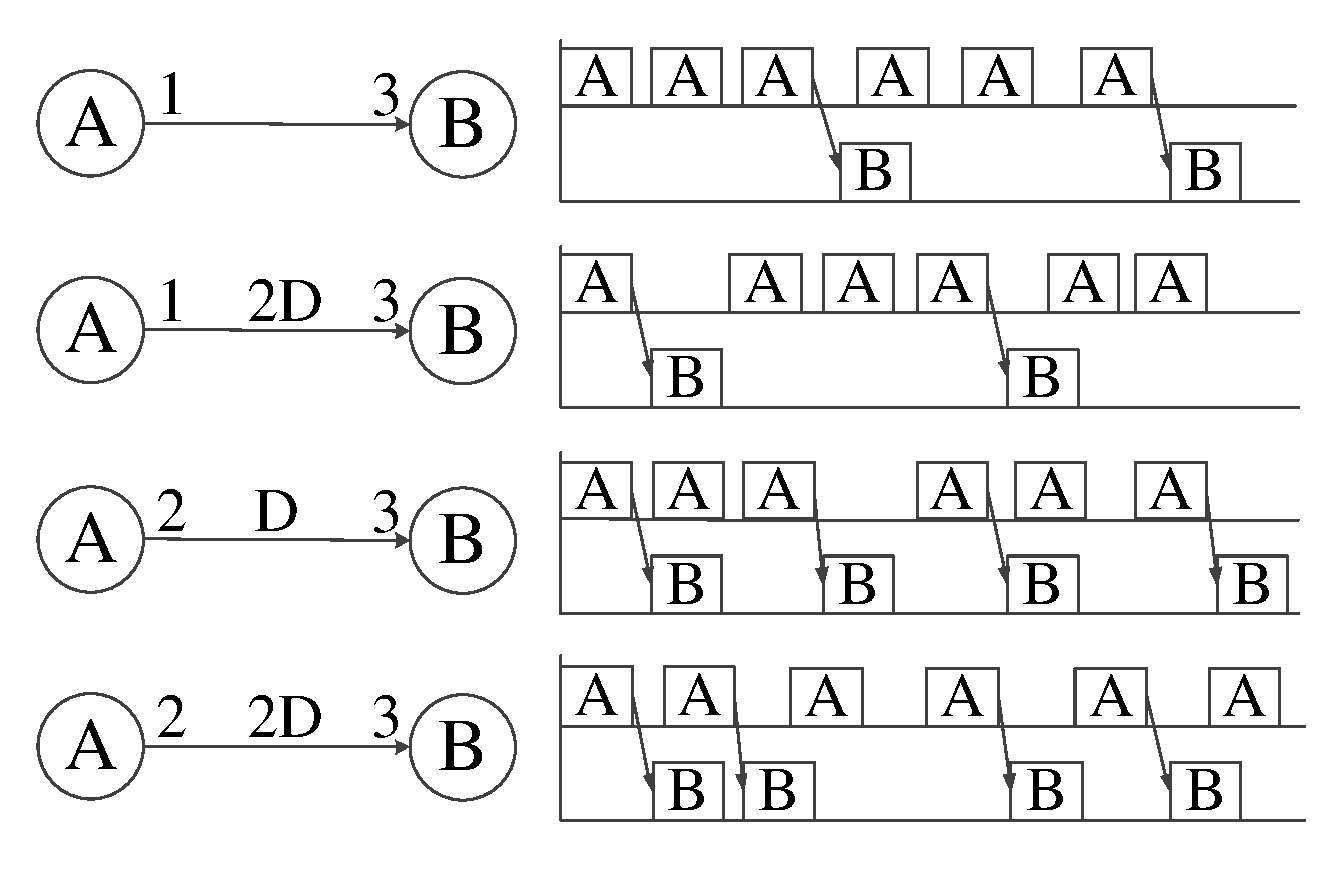
\includegraphics[height=30ex]{figure/SDF-VArc.pdf}\\
  \caption{SDF图中一些弧与优先关系的例子}\label{SDF-fig-VArc}
\end{figure}

从图\ref{SDF-fig-VArc}的例子可以看出,SDF 中不同的弧就对应了所连接两任务之间不同的制约关系。如果将弧上起点、终点的数字以及弧上的 Delay 都认为是虚拟数据,用这条弧表示一个虚拟数据流,那么该数据流也将决定任务间的一个优先依赖关系。而由于数据是虚拟的,其间并没有真正的数据通信,这样,如果要在已有的 SDF 任务之间加入新的优先依赖关系,那么只用向其中加入对应的虚拟数据流即可。本文称这类含有虚拟数据流的 SDF 为广义同步数据流 (General Synchronous Data Flow, GSDF)。

COSS 算法中对周期性释放时间和时间限的约束都是通过构建虚拟结点并在结点之间赋予特定的虚拟数据流来实现的。

%本算法的优势
\subsection{算法模型的选择}
COSS 算法选择SDF模型是因为SDF具有以下特点:

(1)	通过任务之间数据的产生和消耗值的设定,可灵活构建任务运行次数的比例关系。如$t_i$ -> $t_j$ 产生 m 个数据,消耗 n 个数据,可配比任务间运行频率为 n:m。 此产生和消耗的数据可以是真实的数据,也可是虚拟数据,如果是虚拟数据时,下一步从 DAG 构造静态表时不考虑数据通信的开销,只考虑任务间的运行次数比例及优先关系约束,可灵活实现各种任务间的优先关系。

(2)	将调度过程分为三步,构建 GSDF 图,从 GSDF 到 DAG,再从 DAG 生成静态调度表,也给该算法带来了灵活性。构建 GSDF 图的灵活性如(1)所述;此外,在从 DAG 到静态调度表前,还可根据特殊需求对 DAG 进行改动,使算法的使用范围更广(添加新的约束关系,改变任务间数据通信等)。此外,从 DAG 到静态调度表时任务是否可抢占也是可以灵活掌握的,如可在 DLS 算法中查找时间空隙时直接选取可最早开始的时间空隙,不足以完成任务时可继续使用下一时间空隙,有必要时还可将搜索策略由最早开始时间改为搜索最早结束时间等。


\section{释放时间约束}

在不考虑核间通信延时的情况下,由一个任务集数据依赖关系的SDF描述,可以得到在有限个核上的静态调度表。这离本文的目标还有一定的距离,因为任务的时间约束还没有处理。我们将时间约束分为任务周期性释放的时间约束和任务运行时间限 (deadline) 约束两部分分别处理。
%图\ref{SDF-fig-COSS-steps} 直观的给出目前待解决的问题存在于哪些过程,橙色底色的过程是研究的重点问题。

本节首先来考虑构建GSDF时,任务的周期性释放时间约束如何描述。它包括任务的释放周期$T_i$ 及首次任务释放时间$O_i$两方面。

\subsection{加入释放时间约束的方法}
\label{SDF-time-constraint}

在由任务集T根据约束关系构建SDF时,映射任务间数据依赖的约束关系是一件容易的事情,因为SDF本身就是描述数据在各运算结点间的流向的。首先在图中加入所有运算结点,然后按照SDF中弧的定义,依次加入所有任务间数据流向即可,弧上的数据反映有数据通信需求的任务间运行的频率比例。

下面重点考察周期性约束对SDF图的影响。由于SDF图是纯数据驱动型的,所有结点是否可调度完全取决于通向该结点的数据是否已准备充分,而实时系统中的周期性约束则完全是时间驱动型的。这样,要在SDF 中能处理时间层面上的问题,有必要在SDF中引入反应实际时间信息的单元。因此,考虑在SDF中加入一个虚拟的单位周期任务结点V,它要满足以下两个条件\label{SDF-V-conditions}

(1)	为了能够反映时间,V必须是串行执行的,并且相邻两次运行之间无时间间隔。

(2)	为了反映单位周期,V执行时间必须是1个单位时间。

由此可知V必须有一条自依赖的弧,以保证V的串行执行。从以上两个条件可知,虚拟结点 V 第k 次运行的释放时间为
\begin{equation}\label{SDF-eq-R0k}
  R_0[k]=k-1
\end{equation}
结束时间为
\begin{equation}\label{SDF-eq-F0k}
  F_0[k]=R_0[k]+1=k
\end{equation}

有了单位周期结点V 后,相当于整个SDF系统中有了标准时钟,假设任务$t_i$的释放周期和首次释放时间分别为$T_i$ 和$O_i$,那么只需在虚拟结点V和$t_i$ 结点间加入一条虚拟数据流,弧的起点为1,终点为$T_i$,弧上的 Delay 值设为
\begin{equation}
  \label{SDF-eq-r-time}
  D_{0i}=T_i-O_i
\end{equation}
即可,如图\ref{SDF-fig-time-constraint}所示,从 V 到 $t_i$ 的弧即为所添加的对 $t_i$ 的释放时间约束。

\begin{figure}[!hbt]
  \centering
  % Requires \usepackage{graphicx}
  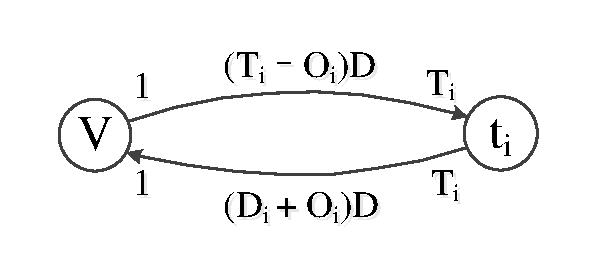
\includegraphics[height=13ex]{figure/SDF-time-constraint.pdf}\\
  \caption{在SDF中为$t_i$添加时间约束}\label{SDF-fig-time-constraint}
\end{figure}

%=======================================================================
%产生两个问题,一个是周期约束与数据约束的一致性问题,另一个如下所述


例如有以下周期性任务集 $T=\{t_1, t_2\}$,周期性时间约束为
\begin{gather*}
  t_1: T_1=2, O_1=0\\
  t_2: T_2=3, O_2=0
\end{gather*}

根据以上方法可以构建GSDF图如图\ref{SDF-fig-r-time}所示。

\begin{figure}[!htb]
  \centering
  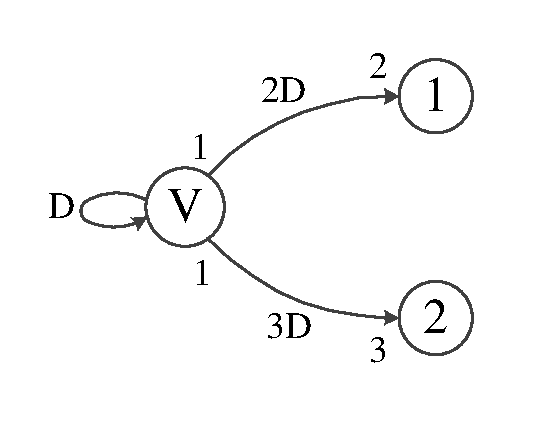
\includegraphics[height=20ex]{figure/SDF-1-r-time.pdf}
  \caption{一组周期性任务加入释放时间约束后得到的GSDF图}
  \label{SDF-fig-r-time}
\end{figure}

由于$O_1=O_2 = 0$,根据 \eqref{SDF-eq-r-time} 式得到两条弧上的 Delay 分别为2D 和3D。 该 GSDF 的拓扑矩阵为
\begin{equation*}
  \Gamma=\begin{bmatrix}
    1 & -2 & 0 \\
    1 & 0 & -3
  \end{bmatrix}
\end{equation*}
由此,根据 \eqref{basic-eq-matrix} 式可以解得周期内最小整数向量为
\begin{equation*}
  q=\begin{bmatrix}
    6 \\
    3 \\
    2
  \end{bmatrix}
\end{equation*}

以下按文献\cite{SDF1987}中的S类算法得到DAG如图\ref{SDF-fig-DAG} 所示。

\begin{figure}[!htb]
  \centering
  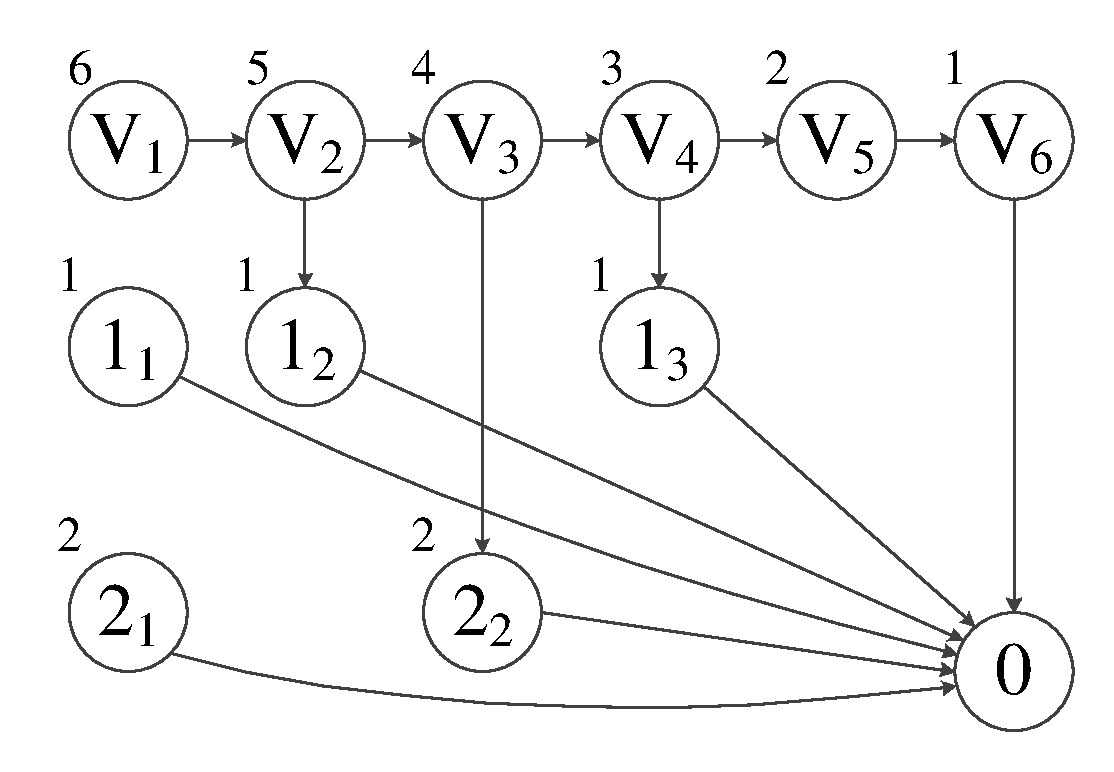
\includegraphics[height=22ex]{figure/SDF-2-DAG.pdf}
  \caption{一组周期性任务根据S类算法得到的DAG图}
  \label{SDF-fig-DAG}
\end{figure}

假设要将此任务集调度到2个处理器上,按照Hu-level的启发式算法\upcite{SDF1987} 可以得到如图\ref{SDF-fig-sch} 的调度结果。

\begin{figure}[!htb]
  \centering
  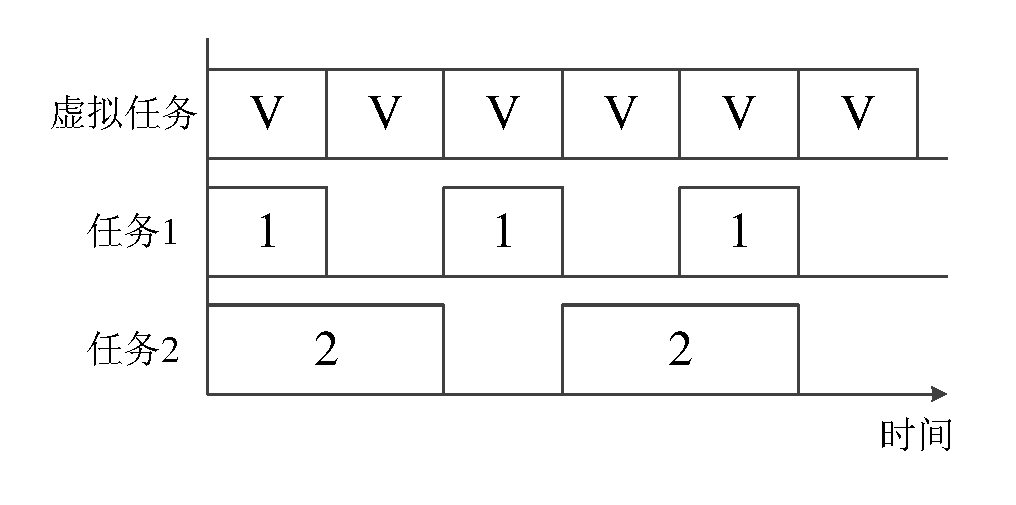
\includegraphics[height=20ex]{figure/SDF-3-sch.pdf}
  \caption{一组周期性任务根据DAG图分配到双核平台上的调度结果}
  \label{SDF-fig-sch}
\end{figure}

可以看到任务1和任务2分别满足了各自的周期性约束条件。

\subsection{加入时间约束的影响}
\label{SDF-time-constraint-influence}

加入时间约束会带来两个问题,首先是虚拟结点造成的影响,其次是关于时间约束与数据约束的一致性问题,以下分别讨论。

(1)加入虚拟结点产生的影响是,按正常调度算法将虚拟结点和其他普通运算结点一起调度的话,势必会使虚拟结点占用正常处理器的运算资源,而实际上这些都是闲置的。因此,在从DAG到生成静态调度表的过程中,也需对虚拟结点特殊处理,这将会在\ref{DLS-virtual-node}节详细论述。

(2)由于表述任务间数据关系的 SDF 图本身即表明了任务之间运行次数的比例关系,例如任务 A 到 B 的依赖关系中,A 每次产生 3 个数据,B 每次消耗 2 个数据,为了保证数据传输速率一致,两任务在调度周期内的运行次数比一定是 2:3 的关系。这样就要求我们在 A 和 B 上添加的周期性约束也必须符合两任务的运行次数比。例如将两任务的周期设为相同时,时间和数据约束的不一致性将导致任务无法调度。这个要求其实反映了 \ref{SDF-intro} 一节中 \eqref{basic-eq-rank} 式所描述的约束条件。如果任务的时间与数据约束不一致,将造成 GSDF 图的拓扑矩阵无零向量解。

但时间约束相比数据依赖约束并不是冗余的,它在任务之间运行次数比例关系以外对任务的释放与执行时间提出了新的要求。仍旧拿上一段中的例子来考虑,已知任务 A 与 B 在一个调度周期内的运行次数比例是 2:3,但如图 \ref{SDF-fig-consistent-constraint} 所示的两种运行分布都是符合数据依赖关系的,显然任务 $t_1$ 与 $t_2$ 不一定具有周期属性。在 (a) 图中任务 A 的两次运行都紧密排布于调度周期的开始,在 (b) 图中任务 B 的三次运行都处于调度周期的末尾,无论如何划分周期,它们都不可能成为周期运行的。

\begin{figure}[!hbt]
  \centering
  % Requires \usepackage{graphicx}
  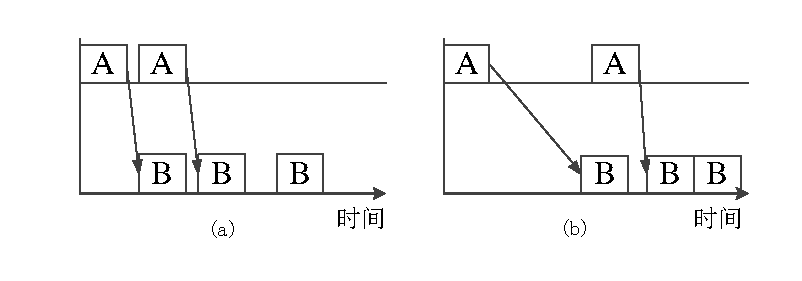
\includegraphics[height=18ex]{figure/SDF-consistent-constraint.pdf}\\
  \caption{SDF 中相同数据约束下的不同时间调度结果}\label{SDF-fig-consistent-constraint}
\end{figure}

但如果将任务 B 加入周期时间约束,就会产生类似图 \ref{SDF-fig-consistent-constraint-2} 所示调度结果,其中 B 在调度周期内仍均匀分布于三个小周期内,即同时符合了周期性与数据依赖关系。

\begin{figure}[!hbt]
  \centering
  % Requires \usepackage{graphicx}
  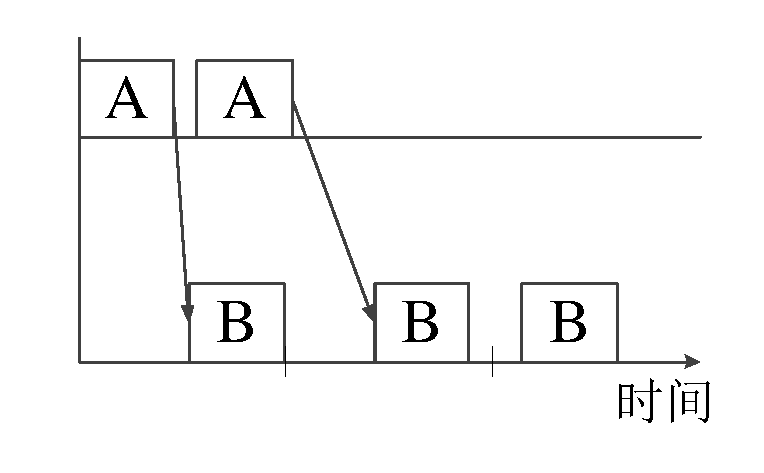
\includegraphics[height=15ex]{figure/SDF-consistent-constraint-2.pdf}\\
  \caption{SDF 中相同数据约束下的周期约束调度结果}\label{SDF-fig-consistent-constraint-2}
\end{figure}

综上所述,在 SDF 中添加周期约束是有必要的,且应与数据约束保持一致性。

\subsection{正确性证明}

下面对\ref{SDF-time-constraint}节所述方法的正确性给出证明。

%\emph{TODO}: 给出证明(待补全)
% 中期报告 + 英文小论文
由周期性任务时间限的定义可知,任务$t_i$第k次运行的释放时间为
\begin{equation}\label{SDF-eq-Rik}
  R_i[k]=(k-1)T_i+O_i
\end{equation}
根据 \eqref{basic-eq-d} 式可知,$t_i$的第k次运行依赖于虚拟结点的前
\begin{equation}\label{SDF-eq-di0k}
  d_{i0}[k]=\left\lceil\frac{T_ik-D_{0i}}{1}\right\rceil=(k-1)T_i+O_i
\end{equation}
次执行。再由 \eqref{SDF-eq-F0k} 式可知虚拟结点前 $d_{i0}[k]$ 次运行结束的时间为
\begin{equation}\label{SDF-eq-F0di0k}
  F_0[d_{i0}[k]]=d_{i0}[k]=(k-1)T_i+O_i
\end{equation}

从 \eqref{SDF-eq-Rik} 和 \eqref{SDF-eq-F0di0k} 式可以看出,$R_i[k]$ 与 $F_0[d_{i0}[k]]$ 相等,也即是说虚拟结点前 $d_{i0}[k]$ 次运行的结束的时间与任务 $t_i$ 第 k 次运行的释放时间相同,因此说明按前述方法在 GSDF 中加入的弧正确反映了任务 $t_i$ 在释放时间上的约束关系。



\section{时间限约束}

\subsection{加入时间限约束的方法}

时间限的约束相比周期性约束理解起来要复杂些。为了保证任务能够在规定时间内完成,仍然要将任务与作为系统时钟的虚拟结点V相联系,但这次需要使V限制任务的结束时间,因此需要从任务结点 $t_i$ 向虚拟结点 V 构建反向弧的制约关系。但这样只是有可能在生成静态调度表时使V在虚拟处理器的调度后移,虚拟处理器上对 V 的调度产生间隙,从而使 V 失去了作为系统时钟的功能。因此需要在下一阶段由DAG产生静态调度表时采用新的判断算法,一方面必须在满足所有约束条件的情况下将V 安排在虚拟处理器上,另一方面V之间的调度不能产生间隙,否则将不能保证实时任务对时间限约束的满足。

下面讨论具体将时间限约束加入SDF图的算法。假设任务 $t_i$ 的时间约束分别为 $T_i$,$D_i$ 和 $O_i$:在图中加入从结点$t_i$ 到虚拟结点V的弧,起点设为 $T_i$,终点为 1,并将弧上的 Delay 设为
\begin{equation}
  \label{SDF-eq-deadline}
  D_{i0}=D_i+O_i
\end{equation}
如图\ref{SDF-fig-time-constraint}所示,其中从 $t_i$ 到 V 的虚拟数据流即为添加的 $t_i$ 的时间限约束。


如有以下周期性任务集 $T=\{t_1, t_2\}$,周期性时间约束为
\begin{gather*}
  t_1: T_1=2, D_1=2, O_1=0\\
  t_2: T_2=3, D_2=3, O_2=0
\end{gather*}

根据前述方法可以构建 GSDF 图如图\ref{SDF-fig-deadline}所示。

\begin{figure}[!htb]
  \centering
  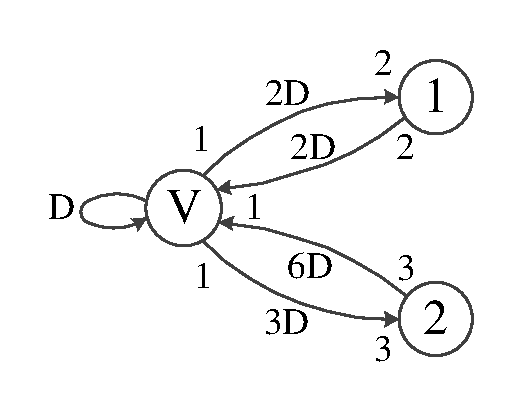
\includegraphics[height=20ex]{figure/SDF-4-deadline.pdf}
  \caption{在SDF图中加入时间限约束}
  \label{SDF-fig-deadline}
\end{figure}

\subsection{正确性证明}

下面证明此方法对实时任务时间限的保证。

%\emph{TODO}: 给出证明(待补全)
% 中期报告 + 英文小论文
由周期性任务时间限的定义可知,任务 $t_i$ 第k次运行的绝对时间限 (absolute deadline) 为
\begin{equation}\label{SDF-eq-Dik}
  D_i[k]=R_i[k]+D_i
\end{equation}

考察虚拟任务的第 $D_i[k]+1$ 次运行,由 \eqref{basic-eq-d} 式可知,它依赖于任务 $t_i$ 的前
\begin{equation}\label{d0iDik}
  d_{0i}[D_i[k]+1]=\left\lceil\frac{(D_i[k]+1)-D_{i0}}{T_i}\right\rceil=k
\end{equation}
次运行,即任务 $t_i$ 的第 k 次运行的结束时间一定不晚于虚拟任务第 $D_i[k]+1$ 次运行的释放时间。而从 \eqref{SDF-eq-R0k} 式可知,虚拟任务第 $D_i[k]+1$ 次运行的释放时间为
\begin{equation}
  R_0[D_i[k]+1]=(D_i[k]+1)-1=D_i[k]
\end{equation}
这与任务 $t_i$ 第 k 次运行的绝对时间限相等。因此,如果虚拟任务能够中间无间隔的被串行调度,那么任务 $t_i$ 的结束时间一定能够满足时间限 (deadline) 的约束。

\section{算法复杂度分析}

本章主要内容是从待调度任务的周期性约束和数据依赖约束生成 GSDF 图,按照以上所述方法,根据任务的周期属性和任务之间的数据依赖属性可直接构建出 GSDF 图中的一个顶点或一条边,因此假设建立图中的一个结点或一条边为一个基本操作。已知任务集中的任务个数为 n,其中周期性任务有 p 个,任务之间的数据依赖关系有 q 个,那么构建的 GSDF 图中,顶点数为 $V_G=n+1$,边数为 $E_G=q+2p$,由此得到总的操作数为
$$\textnormal{Op}=(n+1)+(q+2p)=n+q+2p+1$$
因此构建 GSDF 过程的时间复杂度为
$$O(V_G+E_G)=O(n+q+p)$$

COSS 算法总的复杂度将在\ref{COSS-complexity}节中得到。

\section{任务集的可调度性}
在\ref{SDF-time-constraint-influence}节中可以看到任务的时间和数据约束的不一致性将可能造成任务无法调度。下面讨论可调度任务集的必要条件。

由于 COSS 算法前两步对任务的描述主要采用 GSDF 图,而它在数学特性上与 SDF 是一致的,因此 GSDF 模型对任务集的要求与 SDF 的基本一致,主要有以下几点:
\begin{enumerate}
  \item 数据约束内部,以及数据约束与周期性时间约束之间应当是一致的,如 \ref{SDF-time-constraint-influence} 节所述。其数学上的表述即如 \ref{SDF-intro} 节的 \eqref{basic-eq-rank} 式,要使拓扑矩阵有零向量空间的非零整数解,拓扑矩阵的秩必须是 (结点数-1)。
  \item GSDF 中弧上的 Delay 必须保证任务能够持续运行。如图\ref{SDF-fig-requirement}所示的两个 GSDF,其拓扑矩阵显然满足第1 条约束,但由于弧上的 Delay 不足,导致任务无法启动。
\begin{figure}[!hbt]
  \centering
  % Requires \usepackage{graphicx}
  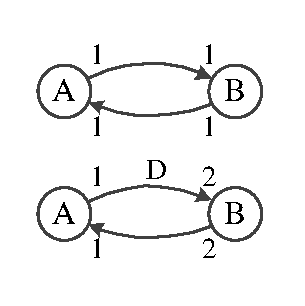
\includegraphics[height=22ex]{figure/SDF-requirement.pdf}\\
  \caption{Delay 不足导致 GSDF 任务无法启动}\label{SDF-fig-requirement}
\end{figure}

  \item \ref{SDF-time-constraint}节中对虚拟结点的约束也反映在任务的时间属性中。虚拟结点要求被串行且无间隔的调度,这要求在 GSDF 转化为 DAG 之后,所有虚拟结点的 SBL 以 1 为单位依次递减。如果虚拟结点的 SBL 值出现断层,则说明一定有任务在这些虚拟结点对应时间内的运行超过了时间限制,从而无法调度。
\end{enumerate}

任务集可调度的充分条件需要考虑目标平台的具体特征,如处理器的个数、连接情况、处理器之间传输速率等要素,无法确切得出,即使本调度算法对某一任务集无法找到有效调度,也不能下结论该任务集是不可调度的,可能存在有效调度只是算法没有找到,毕竟 DAG 的调度算法部分仅是一个启发式的算法,无法对所有可能的调度方案都一一搜索,那将会是 $O(n^m)$ 的复杂度。

\section{本章小结}

本章首先对 COSS 算法的总体设计给出了说明,包括要解决的问题模型、总体算法流程、研究过程中可能遇到的难点,并总结了 COSS 算法的优势所在。其次,本章第2节探讨了算法的构思过程,并论述了从几种并行计算模型中选择 SDF 模型作为算法切入点的原因,在此基础上提出了广义同步数据流模型,为在 SDF 图中灵活添加新的优先约束提供了条件。最后,本章从周期性任务的释放时间和时间限约束两方面分别论述了向 SDF 加入时间约束,构建 GSDF 图的方法,对方法的正确性给出了证明,并分析了算法的复杂度。

